% !TeX spellcheck = it_IT
% !TeX program = pdflatex
%
% LuxSleek-CV 1.1 LaTeX template
% Autore originale: Andreï V. Kostyrka, University of Luxembourg
% Traduzione e adattamento: Nicolò Favagrossa

\documentclass[11pt, a4paper]{article} 

\usepackage[T1]{fontenc}      % Utilizzo di pdfLaTeX
\usepackage[utf8]{inputenc}   
\usepackage[italian]{babel}   % Lingua impostata su italiano
\usepackage{fontawesome5}
\usepackage[left = 0mm, right = 0mm, top = 0mm, bottom = 0mm]{geometry}
\usepackage[stretch = 25, shrink = 25, tracking=true, letterspace=30]{microtype}  
\usepackage{graphicx}         % Per inserire immagini
\usepackage{xcolor}           % Per i colori
\usepackage{marvosym}         % Icone contatti

\usepackage{enumitem}         % Spaziatura liste
\setlist{parsep = 0pt, topsep = 0pt, partopsep = 1pt, itemsep = 1pt, leftmargin = 6mm}

\usepackage{FiraSans}         % Carattere sans-serif
\renewcommand{\familydefault}{\sfdefault}

\definecolor{cvblue}{HTML}{304263}

%%%%%%% DEFINIZIONI COMANDI UTENTE %%%%%%%%%%%%%%%%%%%%%%%%%%%
\newcommand{\dates}[1]{\hfill\mbox{\textbf{#1}}} 
\newcommand{\is}{\par\vskip.5ex plus .4ex} 
\newcommand{\smaller}[1]{{\small$\diamond$\ #1}}
\newcommand{\headleft}[1]{\vspace*{3ex}\textsc{\textbf{#1}}\par%
    \vspace*{-1.5ex}\hrulefill\par\vspace*{0.7ex}}
\newcommand{\headright}[1]{\vspace*{2.5ex}\textsc{\Large\color{cvblue}#1}\par%
     \vspace*{-2ex}{\color{cvblue}\hrulefill}\par}
%%%%%%%%%%%%%%%%%%%%%%%%%%%%%%%%%%%%%%%%%%%%%%%%%%%%%%%%%%%%

\usepackage[colorlinks = true, urlcolor = white, linkcolor = white]{hyperref}

\begin{document}

% Definizioni di stile
\setlength{\topskip}{0pt}
\setlength{\parindent}{0pt}
\setlength{\parskip}{0pt}
\setlength{\fboxsep}{0pt}
\pagestyle{empty}
\raggedbottom

\begin{minipage}[t]{0.33\textwidth} %% Colonna sinistra
% Rettangolo superiore blu
\colorbox{cvblue}{\begin{minipage}[t][5mm][t]{\textwidth}\null\hfill\null\end{minipage}}

\vspace{-.2ex} 
\colorbox{cvblue!90}{\color{white}  %% BOX SINISTRO
\kern0.09\textwidth\relax
\begin{minipage}[t][293mm][t]{0.82\textwidth}
\raggedright
\vspace*{2.5ex}

\Large Nicolò \textbf{\textsc{Favagrossa}} \normalsize 

% Foto
\null\hfill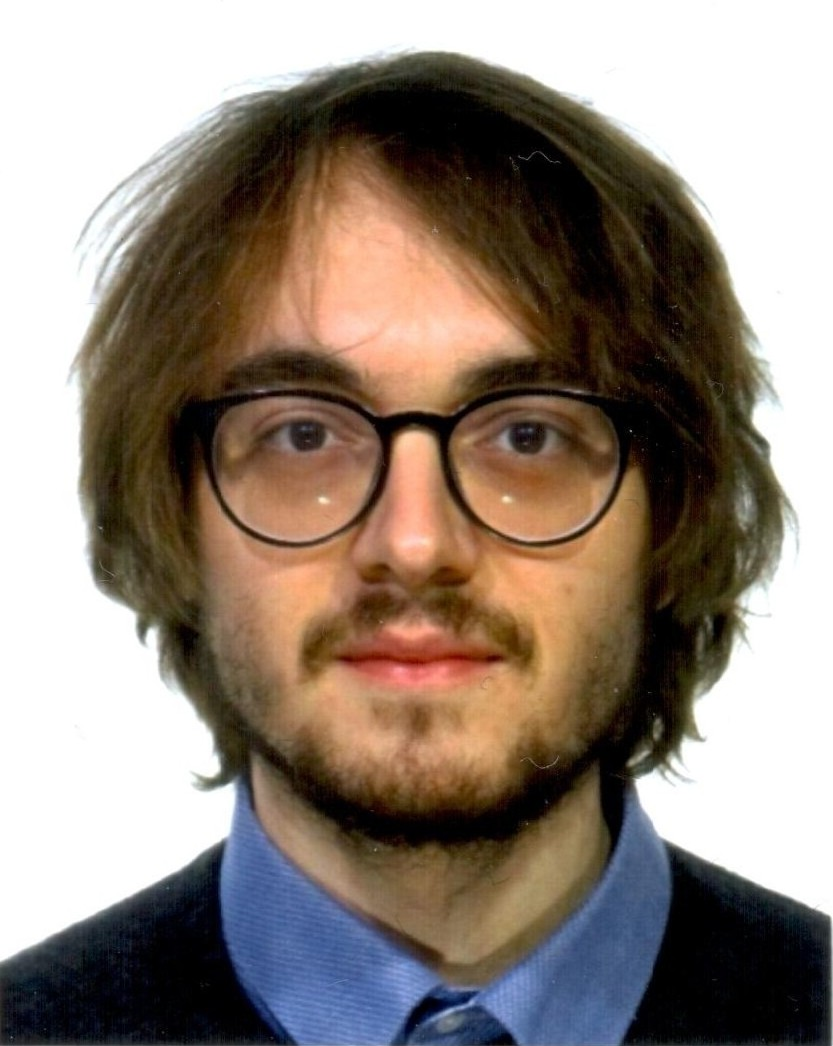
\includegraphics[width=0.65\textwidth]{Fototessera.jpg}\hfill\null

\vspace*{0.5ex}

\headleft{Riassunto}
Studente magistrale in fisica delle particelle elementari e astroparticelle, con oltre 2 anni di esperienza in R\&D nel settore energetico. 

Durante la collaborazione internazionale JUNO, ho maturato una solida competenza nell'analisi dati (C++ e Python), con particolare focus sulla caratterizzazione di rivelatori e sulla riduzione del background.
Nel mio ruolo di tecnico di laboratorio junior, ho sviluppato una spiccata attitudine alla gestione di setup sperimentali e al problem-solving tecnico.


Il mio obiettivo è fondere il rigore accademico con la reattività delle startup in un profilo versatile, pronto a mettere competenze teoriche e sperimentali al servizio di sfide complesse e di frontiera.

\headleft{Contatti}
\small 
\MVAt\ {\small nicolo.favagrossa@gmail.com} \\[0.4ex]
\Mobilefone\ +39\,389\,0155686 \\[0.5ex]
\faLinkedin\ \href{https://www.linkedin.com/in/nicolo-favagrossa/}{Nicolò Favagrossa}\\[0.5ex]
\faGithub\ \href{https://github.com/NicoFava}{NicoFava}
\normalsize

\headleft{Informazioni Personali}
\begin{itemize}
    \item Cittadinanza: \textbf{Italiana}
    \item Lingue: \\
    \textbf{Italiano} (Madrelingua) \\
    \textbf{Inglese C1} (Certificato Universitario) \\
    \item Patente \textbf{B}
\end{itemize}
%\headleft{Soft Skills}
%\begin{itemize}
%\item Comunicazione Scientifica
%\item Analisi Logico-Quantitativa
%\item Gestione e Interpretazione Dati
%\item Problem Solving sotto pressione
%\item Autonomia Decisionale
%\end{itemize}

\end{minipage}%
\kern0.09\textwidth\relax
}
\end{minipage}% 
\hskip2.5em% Margine per l'area bianca
\begin{minipage}[t]{0.56\textwidth}
\setlength{\parskip}{0.8ex}

\vspace{2ex}

\headright{Esperienza Professionale}

\textsc{Junior R\&D Lab Technician} | \textit{Prometheus S.p.A.}\\
\textit{Promosso da Assistant R\&D Technician a Gen 2025}\\ 
\textit{Kilometro Rosso (BG)}\hfill \dates{Nov 2023 – Mag 2026} \\
\smaller{Supporto operativo allo scale-up: transizione dai setup prototipali della fase early-stage all'attuale infrastruttura R\&D presso il Kilometro Rosso.} \\
\smaller{Progettazione e implementazione di campagne sperimentali basate su modelli teorici e ricerca bibliografica attiva.} \\
\smaller{Gestione operativa del laboratorio: approntamento della strumentazione di misura, preparazione di campioni e soluzioni, e ottimizzazione della logistica dei materiali.}\\
\smaller{Sviluppo di strumenti di analisi dati e modelli numerici (Python, C++) per la validazione di fenomeni fisici e calibrazione di sensori.} \\
\smaller{Interfaccia tecnica ("bridge") tra R\&D, partner accademici e investitori tramite comunicazione mirata e redazione di report scientifici.} \\
\smaller{Collaborazione in team multidisciplinari con Senior Nuclear Engineers per la configurazione di strumentazione nucleare e risoluzione di problematiche hardware.}

\headright{Istruzione}

\textsc{Laurea Magistrale in Fisica} \\
\textit{Università degli Studi di Milano} \dates{2025 – Presente} \\
\smaller{Specializzazione: Fisica delle particelle elementari e astroparticelle.}

\is

\textsc{Laurea Triennale in Fisica} \\
\textit{Università degli Studi di Milano} \dates{2020 – 2024} \\
\textit{Voto Finale: 105/110.}\\
\smaller{Titolo della Tesi: Muoni Cosmici in JUNO: Analisi Dati della Fase di Riempimento del Rivelatore}

\headright{Esperienza di Ricerca}
\textsc{Ricercatore Laureando (Tesi Triennale)} | \textit{Collaborazione Internazionale JUNO} \dates{2024} \\
\smaller{Caratterizzazione del flusso di muoni cosmici dai primi dati grezzi del Jiangmen Underground Neutrino Observatory (JUNO) durante la fase critica di riempimento del rivelatore.}\\
\smaller{Sviluppo di un metodo di analisi dati indipendente in C++ (CERN ROOT) per identificare muoni cosmici dai dati grezzi; eseguito benchmarking con gli algoritmi ufficiali JUNO per validare l'efficienza di selezione e la risposta del rivelatore.}\\
\smaller{Analisi statistica e confronto con simulazioni Monte Carlo: misurazione del tasso di muoni e contributo all'ottimizzazione delle strategie di veto per la riduzione del fondo cosmogenico, fondamentale per future misure.}

\headright{Competenze Tecniche}

\smaller{\textbf{Programmazione:} C++ (CERN ROOT), Python, Linux (Bash Scripting), Git/GitHub.} \\
\smaller{\textbf{Analisi Dati \& Statistica:} Metodi Monte Carlo, Fit di verosimiglianza, Analisi delle incertezze, Validazione modelli numerici.} \\
\smaller{\textbf{Elettronica \& Hardware:} Oscilloscopi digitali, Catene di acquisizione, Strumentazione nucleare (PMT, Scintillatori).} \\
\smaller{\textbf{Strumenti:} LaTeX, Microsoft Office, Software DAQ.} \\
\smaller{\textbf{Professionali:} Technical Reporting, Ricerca bibliografica proattiva, Gestione logistica di laboratorio, Teamwork multidisciplinare.}

\end{minipage}

\end{document}